\documentclass[10pt,twocolumn]{article}

\usepackage[letterpaper,margin=0.72in,columnsep=0.18in]{geometry}
\usepackage{times}
\usepackage{microtype}
\usepackage{graphicx}
\usepackage{booktabs}
\usepackage{amsmath,amssymb,amsfonts}
\usepackage{xcolor}
\usepackage{caption}
\usepackage{subcaption}
\usepackage[numbers,sort&compress]{natbib}
\usepackage[hidelinks]{hyperref}

\graphicspath{{figures/}}

% --- compact float / caption spacing (conference look) ---
\captionsetup{font=small,labelfont=bf,skip=3pt}
\captionsetup[subfigure]{font=scriptsize,skip=1pt,labelfont=bf}
\setlength{\textfloatsep}{6pt plus 1pt minus 2pt}
\setlength{\floatsep}{6pt plus 1pt minus 2pt}
\setlength{\intextsep}{6pt plus 1pt minus 2pt}
\setlength{\abovecaptionskip}{3pt}
\setlength{\belowcaptionskip}{0pt}
\setlength{\abovedisplayskip}{4pt}
\setlength{\belowdisplayskip}{4pt}
\setlength{\parskip}{0pt}
\setlength{\parindent}{11pt}
\renewcommand{\topfraction}{0.95}
\renewcommand{\bottomfraction}{0.9}
\renewcommand{\textfraction}{0.05}
\renewcommand{\floatpagefraction}{0.9}
\setcounter{topnumber}{5}
\setcounter{totalnumber}{8}

\title{\vspace{-0.6em}GALA-WM: Residual Action-Conditioned Latent Dynamics\\for Human Motion World Models\thanks{Code: \url{https://github.com/yanghhx/gala-motion}}}
\author{Anonymous\\
\small \url{https://github.com/yanghhx/gala-motion}}
\date{}

\begin{document}
\maketitle
\vspace{-1.0em}

\begin{abstract}
World models let agents ask what will happen under hypothetical actions, yet most human motion systems remain open-loop text-to-motion generators.
We present GALA-WM, an action-conditioned latent world model for human locomotion.
Starting from a frozen motion tokenizer, we learn residual dynamics driven by explicit root commands and plan with latent CEM, following the architectural protocol of DINO-WM while operating on motion latents rather than visual features.
A central design is to modulate and gate the residual by the action, so that null actions collapse toward a copy-last baseline and control becomes necessary rather than optional.
On HumanML3D, GALA-WM improves multi-step prediction over naive dynamics and raises goal-reaching success over a hold planner, yielding a locomotion simulator instead of another text-conditioned synthesizer.
\end{abstract}

\section{Introduction}

World models answer ``what happens if I act''~\cite{ha2018world,hafner2025dreamerv3,lecun2022path}.
Closed-loop benchmarks such as World-in-World~\cite{zhang2026worldinworld} show that visual fidelity does not imply task utility.
Human motion generation has the same gap: MDM~\cite{tevet2023mdm}, TEMOS~\cite{petrovich2022temos}, MotionDiffuse~\cite{zhang2024motiondiffuse}, and MoMask~\cite{guo2024momask} map text to a full clip, with no action interface, no counterfactual rollout, and no planner.

We freeze a GALA tokenizer on HumanML3D~\cite{guo2022humanml3d} and train only dynamics.
Code is at \url{https://github.com/yanghhx/gala-motion}.
\textbf{Claim:} residual action-conditioned latents should beat copy-last / zero / shuffle on multi-step MPJPE, fork under reversed locomotion, and improve CEM over hold.

\paragraph{Contributions.}
(1)~Recast a T2M VAE as a DINO-WM-style simulator (Fig.~\ref{fig:arch}).
(2)~FiLM + action gate so $a{=}0\approx$ copy-last, widening the GT--zero gap.
(3)~Closed-loop diagnostics (MPJPE, action swap, CEM vs hold), not FID~\cite{ebert2018visual,hafner2019planet,zhou2024dinowm}.

\section{Related work}

\paragraph{Latent world models.}
Dreamer / PlaNet / MuZero~\cite{hafner2020dreamerv2,hafner2025dreamerv3,hafner2019planet,schrittwieser2020muzero}, TD-MPC~\cite{hansen2022tdmpc,hansen2024tdmpc2}, and transformer WMs~\cite{seo2023masked,micheli2023transformers,robine2023transformer} learn $p(z_{t+1}\mid z_{\le t},a_t)$.
DINO-WM~\cite{zhou2024dinowm} freezes DINOv2~\cite{oquab2024dinov2} and plans with CEM---our architecture and planner template.
DIAMOND / Genie / Cosmos~\cite{alonso2024diamond,bruce2024genie,nvidia2025cosmos} target pixels; we stay in a $256$-D motion latent~\cite{assran2023vjepa,moerland2023modelbased}.

\paragraph{Motion \& humanoids.}
Puppeteer / HWM~\cite{hansen2024puppeteer,ali2025hwm} and physics controllers~\cite{peng2018deepmimic,won2022physics,ling2020character,luo2023perpetual,rempe2021humor,yuan2023physdiff} need a simulator API.
T2M models~\cite{tevet2023mdm,chen2023executing,zhang2023remodiffuse,jiang2024motiongpt,shafir2024human} optimize $p(x\mid\text{text})$.
We use HumanML3D locomotion~\cite{guo2022humanml3d,mahmood2019amass,punnakkal2021babel,loper2015smpl} as a cheaper proxy.
Baselines are protocols (Table~\ref{tab:provenance}), not competing codebases~\cite{mathieu2016video,oh2015action,finn2016unsupervised,rubinstein1999cem}.

\begin{table}[ht]
\centering
\vspace{-0.2em}
\caption{Baseline provenance.}
\label{tab:provenance}
\scriptsize
\setlength{\tabcolsep}{3pt}
\begin{tabular}{@{}lll@{}}
\toprule
Report & From & Not a reimpl.\ of \\
\midrule
Copy-last & DINO-WM;~\cite{mathieu2016video} & MDM FID \\
Zero / shuffle $a$ & Vis.\ Foresight; Genie & Puppeteer \\
Hold / CEM & DINO-WM / PlaNet & DreamerV3 \\
\bottomrule
\end{tabular}
\vspace{-0.6em}
\end{table}

\section{Method}

\paragraph{Model.}
Frozen GALA maps $x_{1:T}\!\in\!\mathbb{R}^{T\times 263}$ to $\mu\!\in\!\mathbb{R}^{L\times 256}$~\cite{kingma2014vae,loper2015smpl} (Fig.~\ref{fig:arch}a).
Action $a_\ell\in\mathbb{R}^{4}$ is the mean of root channels over four frames.
Residual dynamics (Fig.~\ref{fig:arch}b):
\begin{equation}\vspace{-0.3em}
\hat\mu_{t+1}=\mu_t+\sigma\bigl(g(a_t)\bigr)\,\Delta(\mu_{t-k:t},a_t),\vspace{-0.3em}
\end{equation}
with FiLM~\cite{perez2018film} and a Transformer~\cite{vaswani2017attention,dosovitskiy2021vit}; $a{=}0$ collapses toward copy-last.
Train with $H{=}8$ unroll + decoded pose loss.
CEM (Fig.~\ref{fig:arch}c): pop~48, 8~iters, cost $\|\hat\mu_H-\mu^\star\|^2+0.35\cdot\mathrm{mean}_h\|\hat\mu_h-\mu^\star\|^2$~\cite{rubinstein1999cem,zhou2024dinowm}; hold repeats $z_t$.

\paragraph{Eval.}
Val $n{=}92$; horizons $\{1,4,8\}$ ($\approx\!0.2/0.8/1.6$\,s); denormalized MPJPE; swap $(v_x,v_z)$; CEM success if MPJPE $<80$\,mm and root XY $<0.5$\,m.

\begin{figure*}[t]
\centering
\vspace{-0.4em}
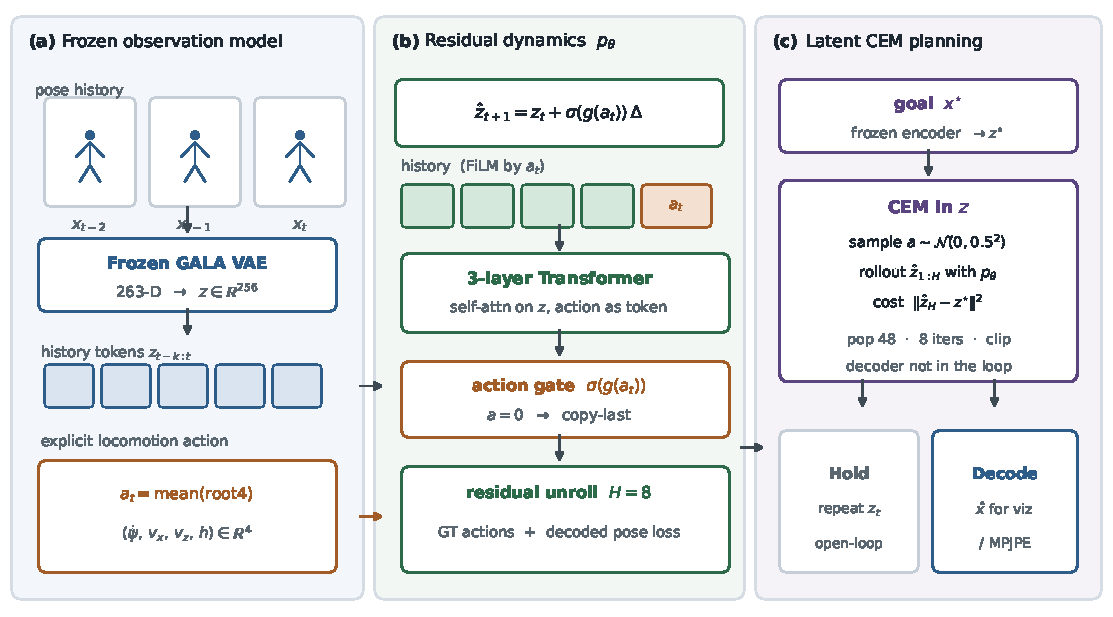
\includegraphics[width=\textwidth]{fig1_architecture.pdf}
\vspace{-0.4em}
\caption{\textbf{GALA-WM} follows the DINO-WM three-block layout~\cite{zhou2024dinowm}.
(a)~Frozen motion VAE.
(b)~Residual Transformer with FiLM and an action gate.
(c)~Latent CEM; the decoder is used only for visualization and MPJPE.}
\label{fig:arch}
\vspace{-0.4em}
\end{figure*}

\section{Experiments}

\textbf{Setup.} HumanML3D~\cite{guo2022humanml3d}; batch~8, AdamW $2{\times}10^{-4}$, bf16, RTX~4060.
Unfixed: absolute 1-step. v1: residual. v2: FiLM+gate+$H{=}8$.

\subsection{Open-loop prediction}
v2+GT is lowest at every horizon (Fig.~\ref{fig:quant}a, Table~\ref{tab:main}); shuffle exceeds copy-last.
FiLM+gate pushes zero/shuffle toward copy-last while GT stays low (Fig.~\ref{fig:quant}b).
@8: $-23.7$\,mm vs copy-last; GT--zero gap $10\!\rightarrow\!22$\,mm (v1$\rightarrow$v2).

\begin{figure}[t]
\centering
\vspace{-0.3em}
\begin{subfigure}[t]{0.49\columnwidth}
\centering
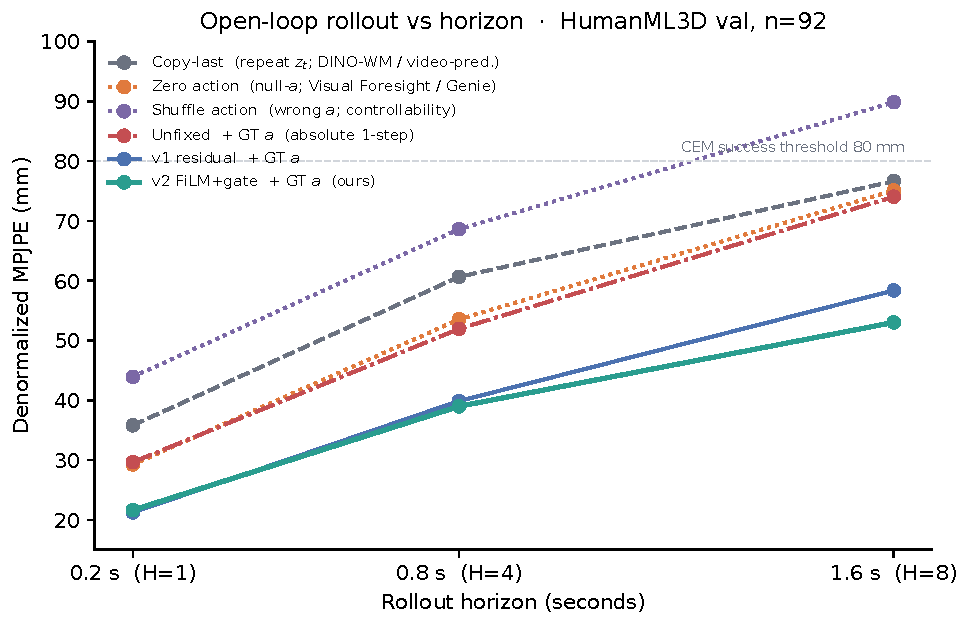
\includegraphics[width=\linewidth,height=2.55cm,keepaspectratio]{fig2_horizon_mpjpe.pdf}
\caption{Horizon MPJPE}
\end{subfigure}\hfill
\begin{subfigure}[t]{0.49\columnwidth}
\centering
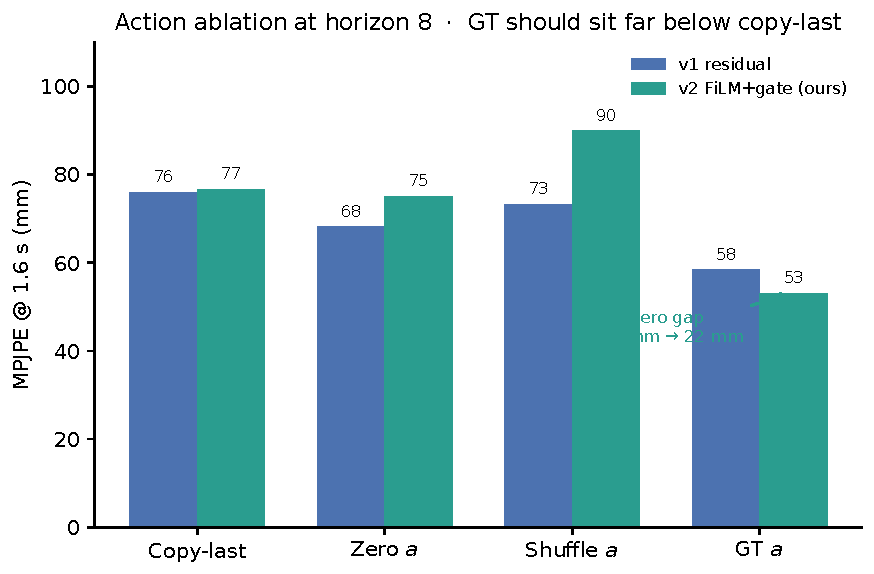
\includegraphics[width=\linewidth,height=2.55cm,keepaspectratio]{fig3_action_ablation.pdf}
\caption{Action ablation}
\end{subfigure}\\[0.2em]
\begin{subfigure}[t]{0.49\columnwidth}
\centering
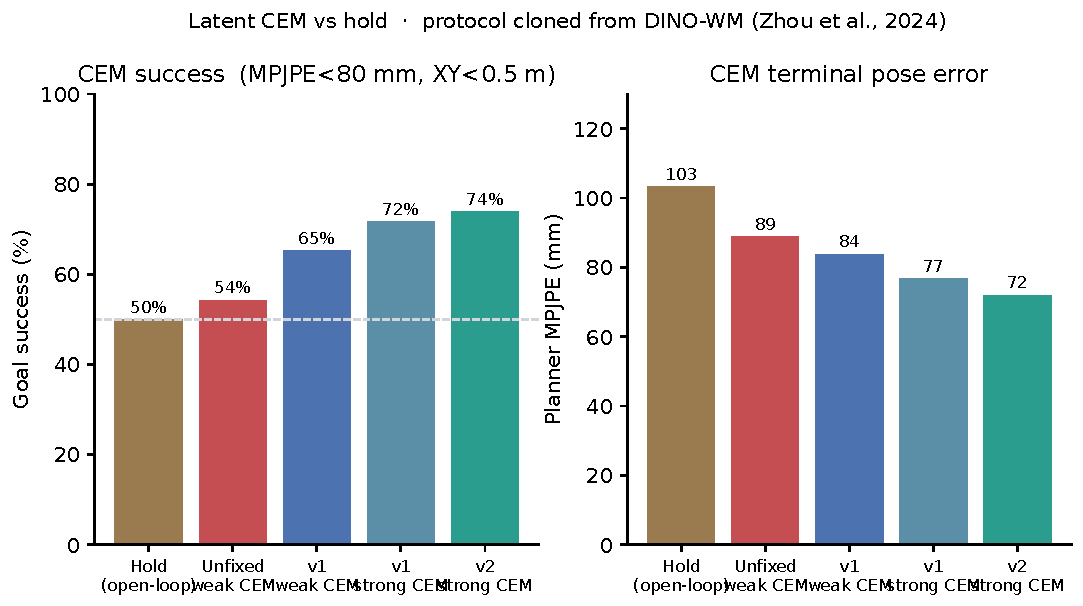
\includegraphics[width=\linewidth,height=2.35cm,keepaspectratio]{fig4_cem.pdf}
\caption{CEM vs hold}
\end{subfigure}\hfill
\begin{subfigure}[t]{0.49\columnwidth}
\centering
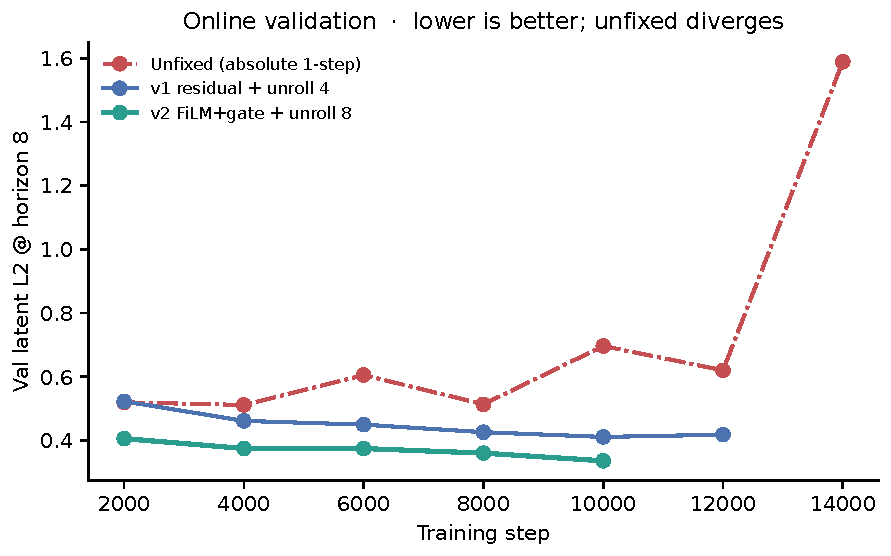
\includegraphics[width=\linewidth,height=2.35cm,keepaspectratio]{fig5_train_latent.pdf}
\caption{Train @ $H{=}8$}
\end{subfigure}
\vspace{-0.3em}
\caption{Quantitative diagnostics ($n{=}92$).}
\label{fig:quant}
\vspace{-0.8em}
\end{figure}

\begin{table}[t]
\centering
\caption{Main results. MPJPE in mm; planning on the right.}
\label{tab:main}
\scriptsize
\setlength{\tabcolsep}{2.8pt}
\begin{tabular}{@{}lcccccc@{}}
\toprule
Method & @1 & @4 & @8 & $\Delta$XY & CEM\% & Hold\% \\
\midrule
Copy-last / Hold & 35.8 & 60.6 & 76.7 & -- & -- & 50 \\
Unfixed & 29.7 & 51.9 & 74.1 & 0.46 & 54.3 & 50 \\
v1 residual & 21.5 & 39.9 & 58.2 & 0.58 & 65.2$^\dagger$ & 50 \\
\textbf{v2 FiLM/gate} & \textbf{21.6} & \textbf{39.0} & \textbf{53.0} & \textbf{0.62} & \textbf{73.9} & 50 \\
\midrule
v2 + zero $a$ & 29.3 & 53.5 & 75.1 & & & \\
v2 + shuffle $a$ & 43.9 & 68.6 & 89.9 & & & \\
\bottomrule
\end{tabular}\\[-0.2em]
{\scriptsize $^\dagger$weak CEM 65.2\%; strong CEM on v1 reaches 71.7\% / 76.8\,mm.}
\vspace{-0.8em}
\end{table}

\subsection{Planning \& qualitative}
CEM reaches 73.9\% vs hold 50\% (Fig.~\ref{fig:quant}c).
Fig.~\ref{fig:qual} shows open-loop skeletons and CEM vs hold.

\begin{figure*}[t]
\centering
\vspace{-0.3em}
\begin{subfigure}[t]{0.48\textwidth}
\centering
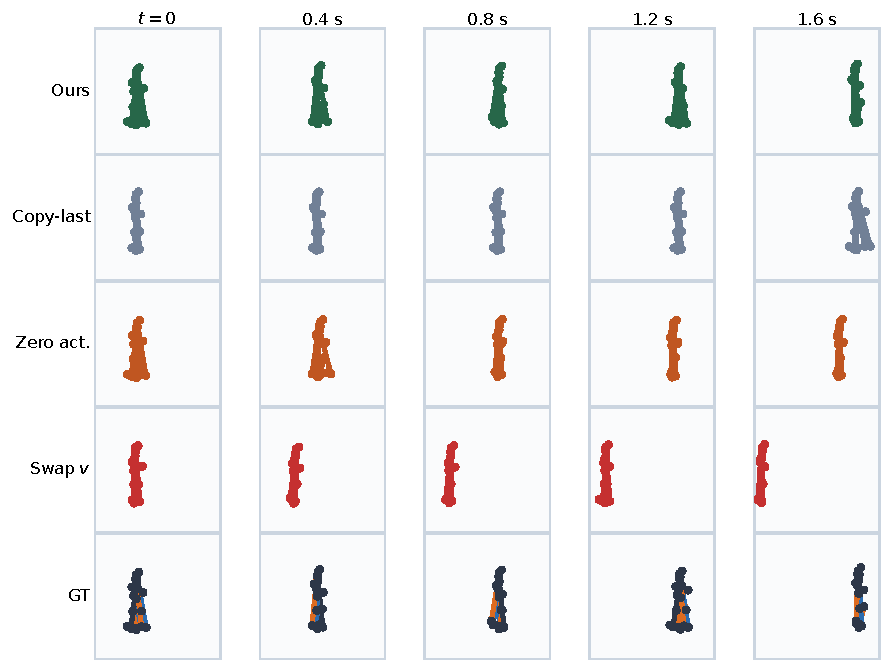
\includegraphics[width=\linewidth]{fig_rollout_grid.pdf}
\caption{Open-loop rollout}
\label{fig:rollout}
\end{subfigure}\hfill
\begin{subfigure}[t]{0.50\textwidth}
\centering
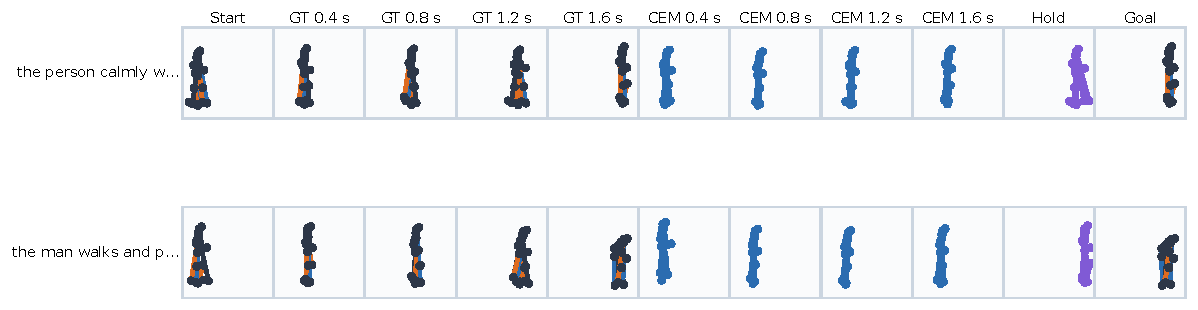
\includegraphics[width=\linewidth]{fig_planning_vis.pdf}
\caption{CEM vs hold}
\label{fig:planvis}
\end{subfigure}\\[0.15em]
\begin{subfigure}[t]{0.42\textwidth}
\centering
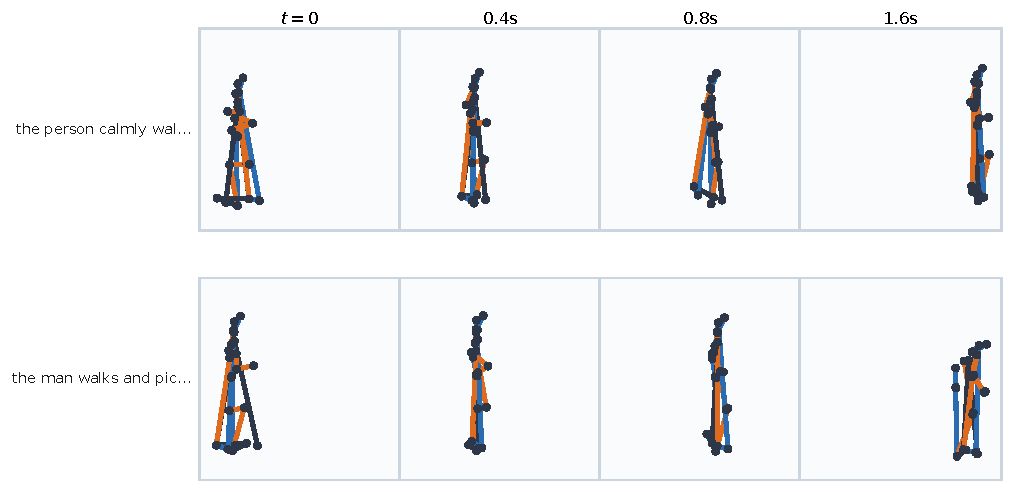
\includegraphics[width=\linewidth,height=2.8cm,keepaspectratio]{fig_dataset_teaser.pdf}
\caption{Domain clips}
\label{fig:data}
\end{subfigure}\hfill
\begin{subfigure}[t]{0.56\textwidth}
\centering
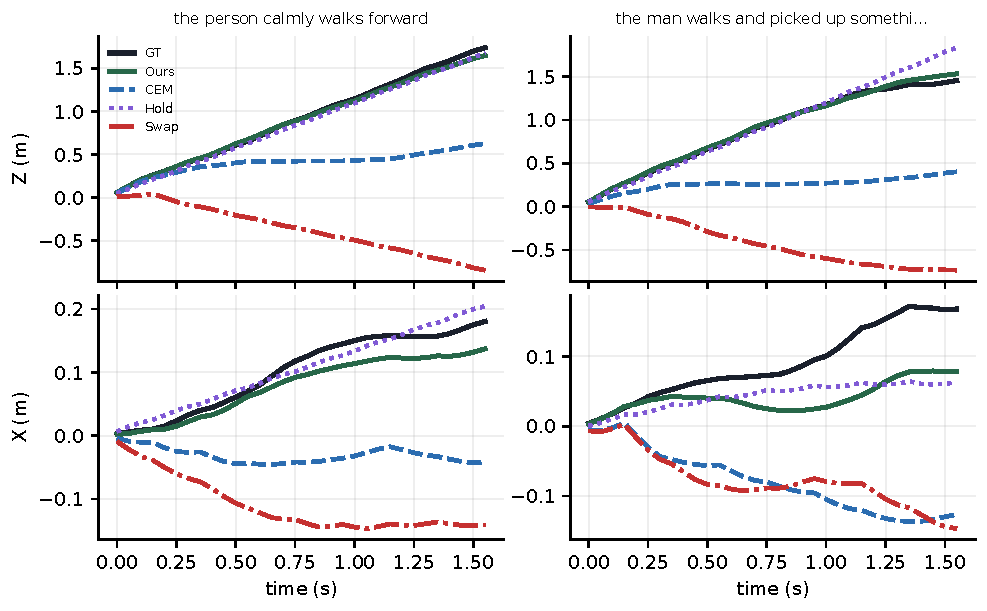
\includegraphics[width=\linewidth,height=2.8cm,keepaspectratio]{fig_planning_xy.pdf}
\caption{Root $Z(t)/X(t)$}
\label{fig:planxy}
\end{subfigure}
\vspace{-0.3em}
\caption{Qualitative results. Decoder used only for visualization.}
\label{fig:qual}
\vspace{-0.5em}
\end{figure*}

\section{Limitations \& conclusion}

Locomotion-centric actions; no physics transfer~\cite{hansen2024puppeteer,zhang2026worldinworld}; 26\% CEM failures; $n{=}92$, one seed.
Residual, action-gated dynamics on a frozen motion VAE yield a DINO-WM-style simulator that beats protocol baselines on prediction and planning~\cite{zhou2024dinowm,black2024pi0,lecun2022path,sutton2018rl}.

\bibliographystyle{unsrtnat}
\bibliography{references}

\end{document}
